%!TeX root=../sensetop.tex
\chapter[Chapter \thechapter]{}
\lettrine[lines=4,lraise=0.3]{T}{he} family of Dashwood had long been settled in Sussex. Their estate was large, and their residence was at Norland Park, in the centre of their property, where, for many generations, they had lived in so respectable a manner as to engage the general good opinion of their surrounding acquaintance. The late owner of this estate was a single man, who lived to a very advanced age, and who for many years of his life, had a constant companion and housekeeper in his sister. But her death, which happened ten years before his own, produced a great alteration in his home; for to supply her loss, he invited and received into his house the family of his nephew Mr Henry Dashwood, the legal inheritor of the Norland estate, and the person to whom he intended to bequeath it. In the society of his nephew and niece, and their children, the old Gentleman’s days were comfortably spent. His attachment to them all increased. The constant attention of Mr and Mrs Henry Dashwood to his wishes, which proceeded not merely from interest, but from goodness of heart, gave him every degree of solid comfort which his age could receive; and the cheerfulness of the children added a relish to his existence.

By a former marriage, Mr Henry Dashwood had one son: by his present lady, three daughters. The son, a steady respectable young man, was amply provided for by the fortune of his mother, which had been large, and half of which devolved on him on his coming of age. By his own marriage, likewise, which happened soon afterwards, he added to his wealth. To him therefore the succession to the Norland estate was not so really important as to his sisters; for their fortune, independent of what might arise to them from their father’s inheriting that property, could be but small. Their mother had nothing, and their father only seven thousand pounds in his own disposal; for the remaining moiety of his first wife’s fortune was also secured to her child, and he had only a life-interest in it.

The old gentleman died: his will was read, and like almost every other will, gave as much disappointment as pleasure. He was neither so unjust, nor so ungrateful, as to leave his estate from his nephew;—but he left it to him on such terms as destroyed half the value of the bequest. Mr Dashwood had wished for it more for the sake of his wife and daughters than for himself or his son;—but to his son, and his son’s son, a child of four years old, it was secured, in such a way, as to leave to himself no power of providing for those who were most dear to him, and who most needed a provision by any charge on the estate, or by any sale of its valuable woods. The whole was tied up for the benefit of this child, who, in occasional visits with his father and mother at Norland, had so far gained on the affections of his uncle, by such attractions as are by no means unusual in children of two or three years old; an imperfect articulation, an earnest desire of having his own way, many cunning tricks, and a great deal of noise, as to outweigh all the value of all the attention which, for years, he had received from his niece and her daughters. He meant not to be unkind, however, and, as a mark of his affection for the three girls, he left them a thousand pounds a-piece.

\begin{figure}[tbph]
\centering
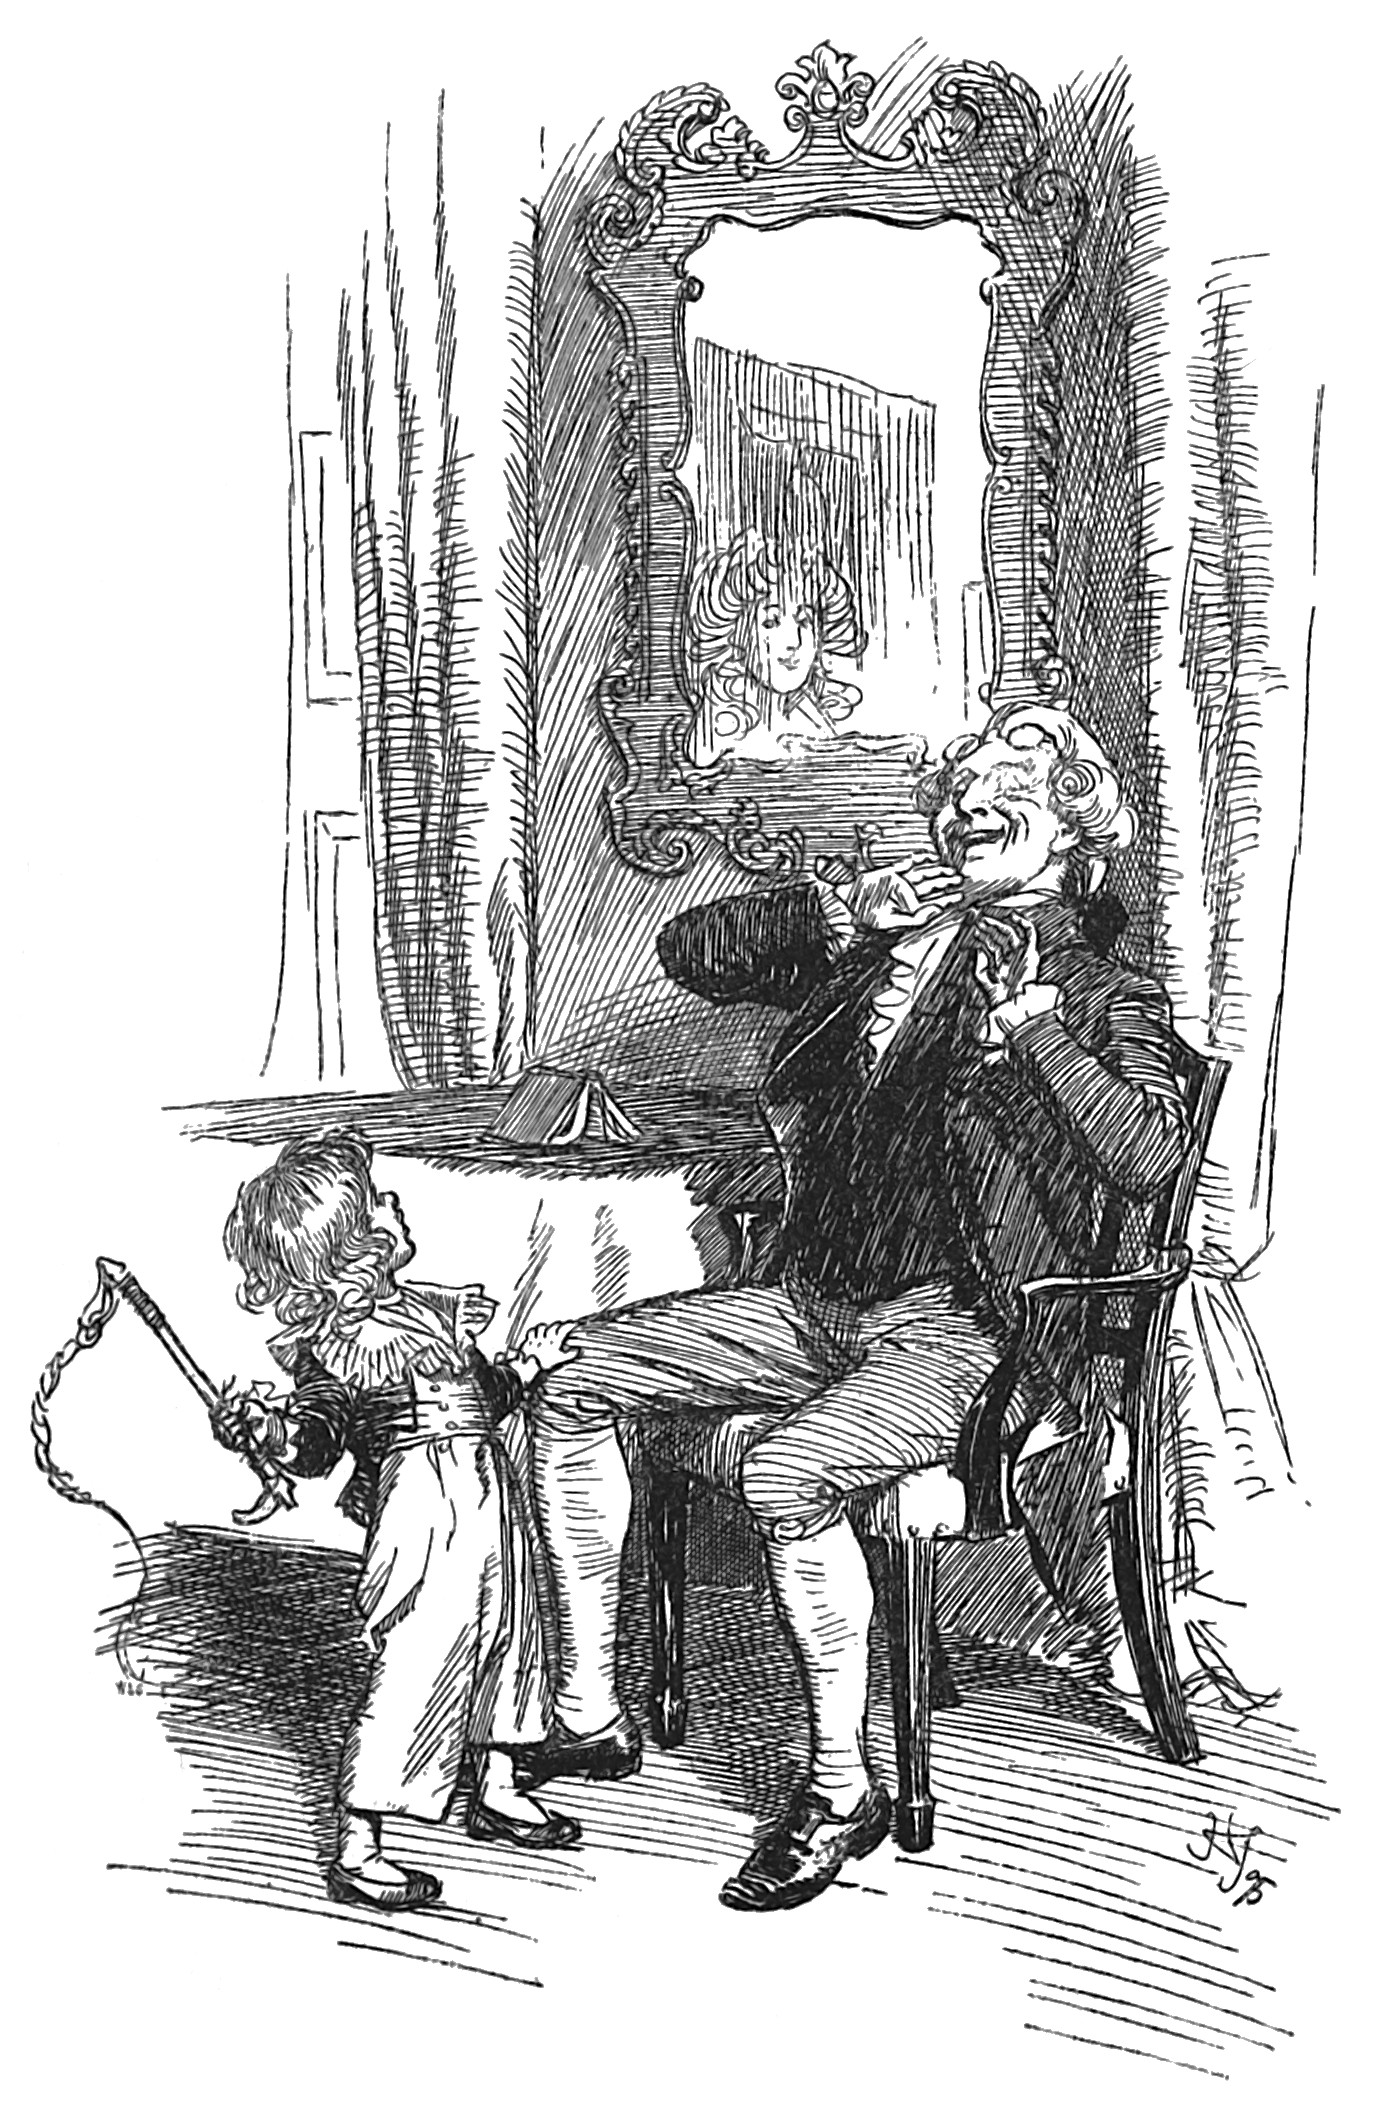
\includegraphics[width=.9\textwidth]{1son}
\caption{His son’s son, a child of four years old}
\end{figure}

Mr Dashwood’s disappointment was, at first, severe; but his temper was cheerful and sanguine; and he might reasonably hope to live many years, and by living economically, lay by a considerable sum from the produce of an estate already large, and capable of almost immediate improvement. But the fortune, which had been so tardy in coming, was his only one twelvemonth. He survived his uncle no longer; and ten thousand pounds, including the late legacies, was all that remained for his widow and daughters.

His son was sent for as soon as his danger was known, and to him Mr Dashwood recommended, with all the strength and urgency which illness could command, the interest of his mother-in-law and sisters.

Mr John Dashwood had not the strong feelings of the rest of the family; but he was affected by a recommendation of such a nature at such a time, and he promised to do every thing in his power to make them comfortable. His father was rendered easy by such an assurance, and Mr John Dashwood had then leisure to consider how much there might prudently be in his power to do for them.

He was not an ill-disposed young man, unless to be rather cold hearted and rather selfish is to be ill-disposed: but he was, in general, well respected; for he conducted himself with propriety in the discharge of his ordinary duties. Had he married a more amiable woman, he might have been made still more respectable than he was:—he might even have been made amiable himself; for he was very young when he married, and very fond of his wife. But Mrs John Dashwood was a strong caricature of himself;—more narrow-minded and selfish.

When he gave his promise to his father, he meditated within himself to increase the fortunes of his sisters by the present of a thousand pounds a-piece. He then really thought himself equal to it. The prospect of four thousand a-year, in addition to his present income, besides the remaining half of his own mother’s fortune, warmed his heart, and made him feel capable of generosity. »Yes, he would give them three thousand pounds: it would be liberal and handsome! It would be enough to make them completely easy. Three thousand pounds! he could spare so considerable a sum with little inconvenience.« He thought of it all day long, and for many days successively, and he did not repent.

No sooner was his father’s funeral over, than Mrs John Dashwood, without sending any notice of her intention to her mother-in-law, arrived with her child and their attendants. No one could dispute her right to come; the house was her husband’s from the moment of his father’s decease; but the indelicacy of her conduct was so much the greater, and to a woman in Mrs Dashwood’s situation, with only common feelings, must have been highly unpleasing;—but in \textit{her} mind there was a sense of honour so keen, a generosity so romantic, that any offence of the kind, by whomsoever given or received, was to her a source of immovable disgust. Mrs John Dashwood had never been a favourite with any of her husband’s family; but she had had no opportunity, till the present, of showing them with how little attention to the comfort of other people she could act when occasion required it.

So acutely did Mrs Dashwood feel this ungracious behaviour, and so earnestly did she despise her daughter-in-law for it, that, on the arrival of the latter, she would have quitted the house for ever, had not the entreaty of her eldest girl induced her first to reflect on the propriety of going, and her own tender love for all her three children determined her afterwards to stay, and for their sakes avoid a breach with their brother.

Elinor, this eldest daughter, whose advice was so effectual, possessed a strength of understanding, and coolness of judgment, which qualified her, though only nineteen, to be the counsellor of her mother, and enabled her frequently to counteract, to the advantage of them all, that eagerness of mind in Mrs Dashwood which must generally have led to imprudence. She had an excellent heart;—her disposition was affectionate, and her feelings were strong; but she knew how to govern them: it was a knowledge which her mother had yet to learn; and which one of her sisters had resolved never to be taught.

Marianne’s abilities were, in many respects, quite equal to Elinor’s. She was sensible and clever; but eager in everything: her sorrows, her joys, could have no moderation. She was generous, amiable, interesting: she was everything but prudent. The resemblance between her and her mother was strikingly great.

Elinor saw, with concern, the excess of her sister’s sensibility; but by Mrs Dashwood it was valued and cherished. They encouraged each other now in the violence of their affliction. The agony of grief which overpowered them at first, was voluntarily renewed, was sought for, was created again and again. They gave themselves up wholly to their sorrow, seeking increase of wretchedness in every reflection that could afford it, and resolved against ever admitting consolation in future. Elinor, too, was deeply afflicted; but still she could struggle, she could exert herself. She could consult with her brother, could receive her sister-in-law on her arrival, and treat her with proper attention; and could strive to rouse her mother to similar exertion, and encourage her to similar forbearance.

Margaret, the other sister, was a good-humoured, well-disposed girl; but as she had already imbibed a good deal of Marianne’s romance, without having much of her sense, she did not, at thirteen, bid fair to equal her sisters at a more advanced period of life.